\begin{figure}[h]
  \centerfloat
  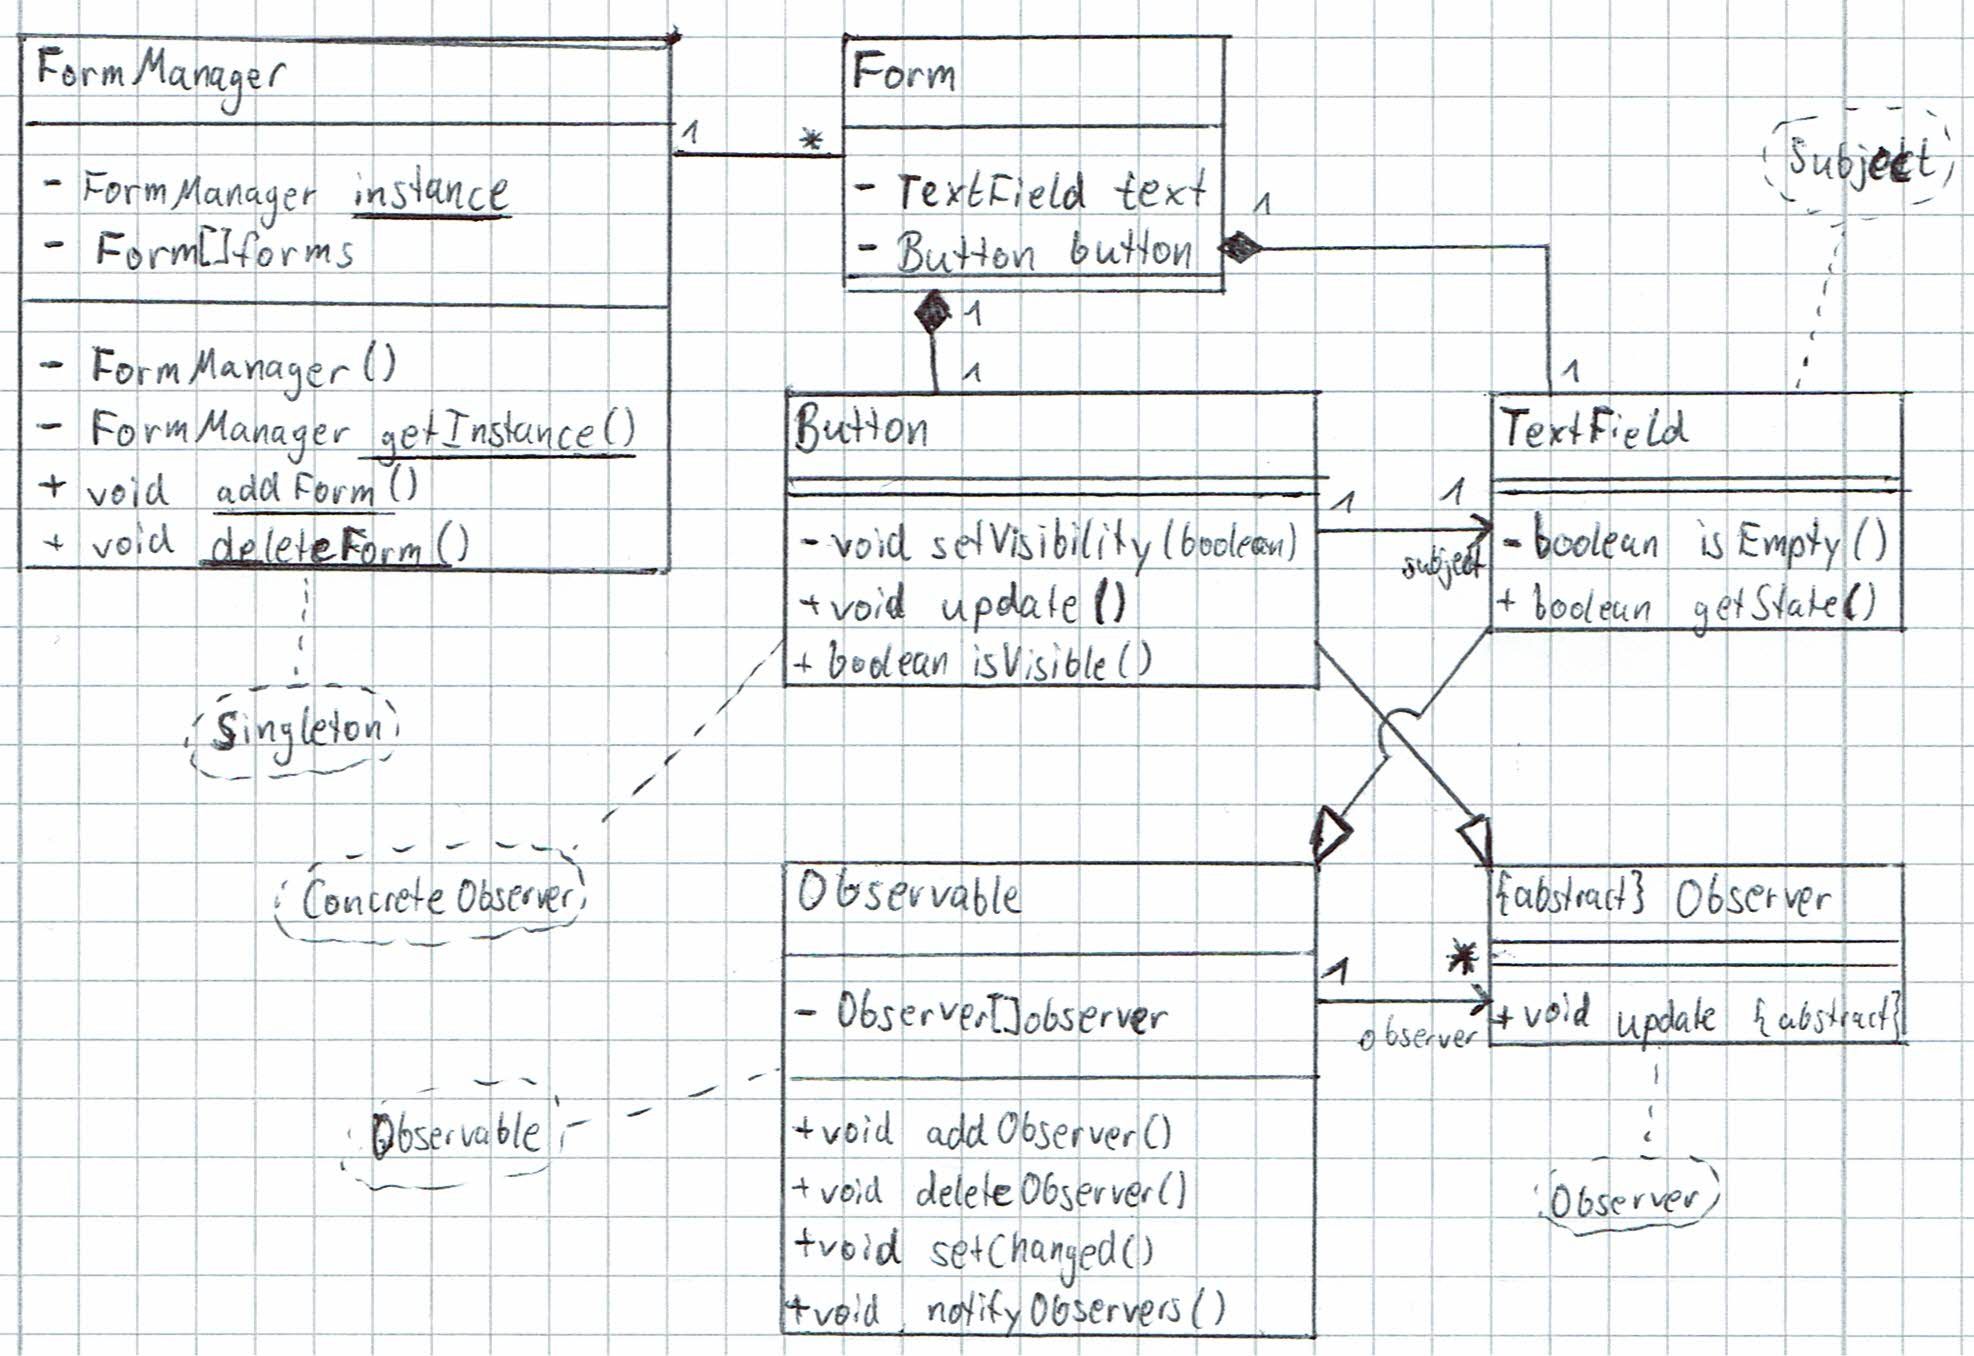
\includegraphics{1_forms}
\end{figure}
Unterstrichene Attribute-/Methodennamen sollen static sein. Die im FormManager public static deklarierten Methoden (addForm(), deleteForm()) sind zum verwalten der Forms da.
Diese delegieren die eigentliche Logik an Funktionen des eigentlichen Singelton-Objekts (welche hier der Übersichtlichkeit halber weggelassen wurden). Da getInstance() nur
von den public static deklarierten Methoden aus aufgerufen werden soll, ist getInstance() private deklariert.\\
Im Allgemeinen kann ein Observable beliebig viele Oberserver haben, in diesem Beispiel ist aber nur von einem Button (ConcreteObserver) und einem Textfeld (Subject) die Rede.
Dies ist so in den Kardinalitäten impliziert.
